\documentclass[a4paper,11pt]{jsarticle}


% 数式
\usepackage{amsmath,amsfonts}
\usepackage{bm}
\usepackage{siunitx}
% 画像
\usepackage[dvipdfmx]{graphicx}
\usepackage{booktabs}


\begin{document}

\title{}
\author{}
\date{\today}


\section{図の電流計は最大定格$1\mathrm{\,\si{\milli \ampere}}$、内部抵抗$100\mathrm{\,\si{\ohm}}$である。この計器を使って多重範囲の電流計・電圧計を設計する。抵抗値$R_{1}\sim R_{4}$を求めなさい。}
\begin{figure}[htbp]
  \centering
  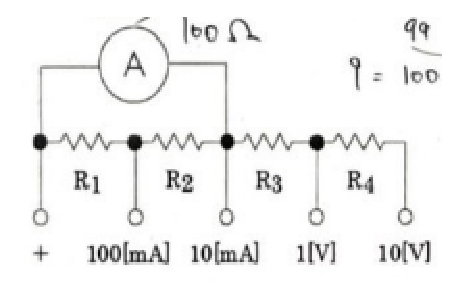
\includegraphics[width=5cm]{fig1.eps}
  \caption{}\label{fig1}
\end{figure}

$[+,\ \mathrm{A_{1}}]$における倍率は$\frac{100}{1}=100$であるため、
\begin{align}
  \begin{split}
    n_{1A}
    &=1+\frac{100+R_{2}}{R_{1}}\\
    100R_{1}
    &=R_{1}+100+R_{2}\\
    99R_{1}-R_{2}
    &=100
    \label{eq1}
  \end{split}
\end{align}

$[+,\ \mathrm{A_{2}}]$における倍率は$\frac{10}{1}=10$であるため、
\begin{align}
  \begin{split}
    n_{2A}
    &=1+\frac{100}{R_{1}+R_{2}}\\
    10R_{1}+10R_{2}
    &=R_{1}+R_{2}+100+R_{2}\\
    9R_{1}+8R_{2}
    &=100
    \label{eq2}
  \end{split}
\end{align}

式\eqref{eq1}$\sim $\eqref{eq2}より、$R_{1}=1.12\mathrm{\,\si{\ohm}},\ R_{2}=11.2\mathrm{\,\si{\ohm}}$となる。

また、
\begin{align}
  \begin{split}
    R_{A}
    &=\frac{R\cdot (R_{1}+R_{2})}{R+R_{1}+R_{2}}\\
    &=\frac{100(1.12+11.2)}{100+1.12+11.2}\\
    &=10.97
    \label{eq3}
  \end{split}
\end{align}
となるから、$[+,\ \mathrm{V_{1}}]$における倍率は$\frac{1}{0.001*100}=10$であるため、
\begin{align}
  \begin{split}
    n_{1V}
    &=1+\frac{R_{3}}{R_{A}}\\
    10\cdot 10.97
    &=10.97+R_{3}\\
    R_{3}
    &=10.97\times 9\\
    &=98.73\mathrm{\,\si{\ohm}}
    \label{eq4}
  \end{split}
\end{align}

$[+,\ \mathrm{V_{2}}]$における倍率は$\frac{10}{0.001*100}=100$であるため、
\begin{align}
  \begin{split}
    100
    &=1+\frac{R_{3}+R_{4}}{R_{A}}\\
    100\times 10.97
    &=10.97+98.79+R_{4}\\
    R_{4}
    &=987.24
    \label{eq5}
  \end{split}
\end{align}


\end{document}